\newpage
\null
\vspace{0.15cm}

\begin{center}
    \Huge{\textbf{\underline{Chapter 1: State Space Search}}}
\end{center}

\setcounter{section}{0}

\vspace{0.35cm}


\section{State Space Search}
\begin{prettyBox}{Definition}{myblue}
State space search does not rely on prior experience. It involves solving a problem by exploring possible states and actions. The process includes:
\begin{enumerate}
    \item \textbf{Modeling the Problem:} Represent the problem using simple or complex data structures.
    \item \textbf{Defining the Search Space:}
        \begin{itemize}
            \item \textbf{Set of States:} Includes the initial state (\(S\)), the goal state (\(G\)), and all intermediate states.
            \item \textbf{Set of Legal Moves:} Represents the actions that allow transitions from one state to another.
        \end{itemize}
    \item \textbf{Defining Functions:}
        \begin{itemize}
            \item \textbf{Movegen(S: state):} Returns a set of states representing the results of all legal moves from the given state.
            \item \textbf{GoalTest(S: state):} Takes a state as input and returns a boolean value, verifying whether the given state is a goal state.
        \end{itemize}
\end{enumerate}
\end{prettyBox}

\vspace{0.35cm}

\begin{prettyBox}{Types of Problems}{myblue}
\begin{itemize}
    \item \textbf{Configuration Problems:} 
    The goal state is not explicitly defined but is identified by its properties. The concept of a path solution is irrelevant; only the goal state is retrieved.
    \item \textbf{Planning Problems:} 
    The goal state is explicitly defined, and the solution involves finding the path to reach the goal state.
\end{itemize}
\end{prettyBox}

\vspace{0.35cm}

\begin{prettyBox}{Note}{red}
Search-based agents are not highly efficient due to the issue of combinatorial explosion. As the search tree grows deeper, the number of nodes increases exponentially, resulting in an unmanageable number of possibilities to explore.
\end{prettyBox}

\vspace{0.35cm}

\begin{prettyBox}{Search Categories}{myblue}
\begin{itemize}
    \item \textbf{Uninformed Search:} Conducted without any guidance or additional data (blind search).
    \item \textbf{Informed Search:} Guided by additional information or heuristics.
\end{itemize}
\end{prettyBox}

\newpage
\subsection*{\underline{Example}}

\vspace{0.5cm}
\begin{prettyBox}{8-Puzzle Problem}{myblue}
The 8-puzzle problem consists of a \(3 \times 3\) matrix with integers from 1 to 8 placed randomly, along with an empty cell represented by \(X\). The goal is to rearrange the matrix to achieve the following configuration:
\end{prettyBox}

\vspace{0.65cm}
\begin{center}
    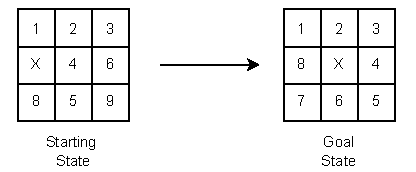
\includegraphics[width=0.6\textwidth]{Chapters/Example/Uninformed/ex1.drawio.pdf}
\end{center}

\vspace{0.45cm}

\begin{prettyBox}{Legal Moves}{myblue}
\begin{itemize}
    \item Slide Up
    \item Slide Down
    \item Slide Right
    \item Slide Left
\end{itemize}
\end{prettyBox}

\vspace{0.45cm}

\begin{prettyBox}{Representation}{myblue}
The matrix can be represented as a 2D array of integers, with the empty cell (\(X\)) optionally represented as \texttt{nil}.
\end{prettyBox}


\vspace{0.35cm}


\begin{prettyBox}{River Crossing Problem}{myblue}
This problem involves a man, a lion, a goat, a cabbage, a boat, and a river. Initially, all entities are on the left side of the river. The goal is to transport all of them to the right side without any entity being harmed:
\begin{itemize}
    \item If the lion and goat are left alone, the lion will kill the goat.
    \item If the goat and cabbage are left alone, the goat will eat the cabbage.
\end{itemize}
\end{prettyBox}


\vspace{0.5cm}
\begin{center}
    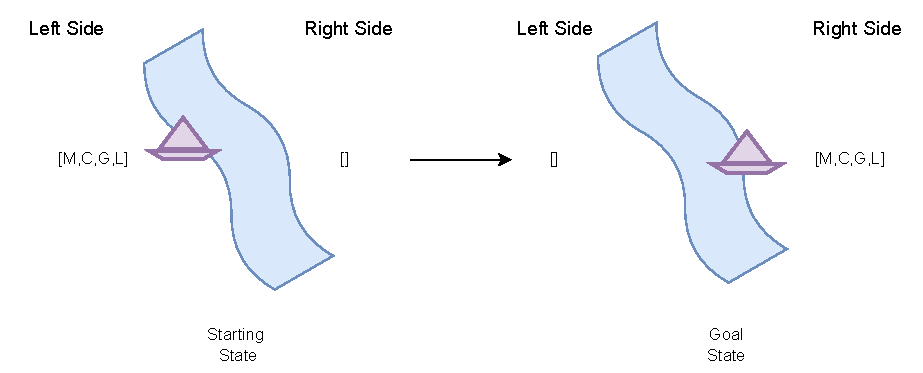
\includegraphics[width=0.8\textwidth]{Chapters/Example/Uninformed/ex2.1.drawio.pdf}
\end{center}

\vspace{0.5cm}
\begin{prettyBox}{Legal Moves}{myblue}
\begin{itemize}
    \item Man takes nothing to the right side.
    \item Man takes the cabbage.
    \item Man takes the lion.
    \item Man takes the goat.
\end{itemize}
\end{prettyBox}

\vspace{0.5cm}
\begin{prettyBox}{Representation}{myblue}
A list of structures, where each structure has the following fields:
\begin{itemize}
    \item \texttt{char name}: The name of the entity (\texttt{'M'} Man , \texttt{'C'} Cabbage, \texttt{'L'} Lion ,\texttt{'G'} Goat).
    \item \texttt{char position}: The position of the entity (\texttt{'L'} Left side, \texttt{'R'} Right side).
\end{itemize}

If any entity is harmed (eaten or killed), it is removed from the list, signifying its destruction.
\end{prettyBox}

\vspace{0.5cm}
\begin{center}
    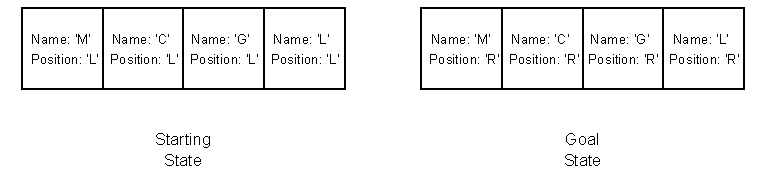
\includegraphics[width=0.8\textwidth]{Chapters/Example/Uninformed/ex2.2.drawio.pdf}
\end{center}

